%!TEX root = ../Thesis.tex
% Chapter Template

\chapter{Development and Testing} % Main chapter title

\label{Development} % Change X to a consecutive number; for referencing this chapter elsewhere, use \ref{ChapterX}

\lhead{Chapter \ref{Development}. \emph{Development and Testing}} % Change X to a consecutive number; this is for the header on each page - perhaps a shortened title

%----------------------------------------------------------------------------------------
%	SECTION 1
%----------------------------------------------------------------------------------------

This chapter will briefly describe the development process of the genetic and clustering algorithms. It will also go into some detail about the design of the algorithm so that the reader may better understand the code and how the algorithms works. This chapter will also be of benefit to those who wish to use the algorithm or even modify it.


\section{Stages of development}

This thesis is built on a project proposal written by \supervisor. The proposal suggested that work could be done to optimize the parameters of the \STC algorithm in order to get better clustering results. The algorithm was already implemented by \supervisor in the programming language Python. In my project draft, a document written in preparation for the master thesis, the problem area was slightly shifted to include the use of a genetic algorithm for optimizing parameters. This necessitated some development and modification of the original implementation.

Because I had no familiarity with Python the \emph{first stage} of development included learning myself the Python programming language. I also had to familiarize myself with the implementation of the \CTC algorithm. The algorithm was implemented with largely hard coded parameters with about one separate module (file) for each parameter configuration. In order to facilitate easier testing of different parameter sets the \emph{second stage} of development involved abstracting the parameter set away so that the clustering function would accept any parameter set. This made it possible to perform initial incremental tests. These incremental tests then informed the design of the genetic algorithm, the \emph{third stage} of development. The genetic algorithm was initially developed to run on a single computer and was designed following the specifications in \cite{Goldberg1989,Negnevitsky2002,Haupt2004a}. Testing of the initial design for the genetic algorithm revealed that it was indeed capable of improving the weighted measure (e-measure) of the clustering results. There were a problem however as testing many chromosomes on a single machine took too much time. It was necessary to distribute the task.

This brings us to the \emph{fourth stage} of development. A small server - client framework was written to facilitate distribution of computation tasks. The genetic algorithm was then rewritten to send chromosomes (essentially parameter sets) to these clients who would then perform the actual clustering tasks. This made it very simple to run the clustering job on multiple CPU cores and multiple computers. Additionally a corpus processor was implemented to convert other corpus files to the snippet format used for the \CTC algorithm. A new subclass of the corpus processor needs to be implemented for each additional corpus to be converted.

One problem with Python 2 is the way it handles memory. The client processes would, at least in some environments, consistently eat up as much memory as they could and never free up memory used. This seemed to be a problem related to the way in which Python 2 allocated and deallocates memory for small variables such as integers. Essentially the Python 2 virtual machine would hold on to memory space allocated to small variables in case it could need such space later. This in essence saves CPU cycles as it does not have to ask for more space later. The problem seemed to be that it did not reuse that space later, but instead opted to ask for a new virtual memory space for small variables. Thus the entire project had to be ported to Python 3.

TODO: Does memory explanation need sources?

\section{Overview of system}
This section will give an overview of the algorithms. It will cover the overall design of the algorithms and diverge briefly into some technical aspects. The entire code base of the project is too big to be covered in the thesis. The code is open source and can be found in it's entirety at \href{http://github.com/snorremd/distributed-clustering}{GitHub - http://github.com/snorremd/distributed-clustering}. The code is licensed under the MIT license and can be used and modified freely. Readers interested in a more detailed look at the implementation are encouraged to take a look at the code and try it out themselves.

\subsection{\CTC}
The original implementation of the \CTC algorithm was authored by \supervisor. The implementation used for this thesis work is more or less the same, but with modifications to allow dynamically specifying parameter sets. The \CTC algorithm is implemented as a class. The class initializer (similar to a constructor) takes as parameters a corpus object, that specifies which corpus is to be used, and a cluster settings object that informs the \CTC object if it is to include singleton ground truth clusters and which value to use for the f-beta-constant for the f-measure. Ground truth clusters are those clusters that only have a single document in it. Including those clusters may make the genetic algorithm favor solutions with many singleton clusters. The f-beta-value determines the relative weight distribution between the precision and recall values used to calculate the f-measure score. Using a very low value for the f-beta score will essentially make the f-measure a measure of precision. Conversely using a very high score will make it a measure of recall. A f-beta value of 1 makes it a harmonious mean of the two. The value can thus be used to tune the kind of results the genetic algorithm optimized for.

The initializer continues by building an index of ground truth clusters, a tag-index, and indexes over different frequency measures (corpus frequency, raw frequency and document frequency) for the terms contained within the corpus. The ground truth index and tag index are both created based on the snippet file specified in the corpus object. The snippet file is marked up in XML and use the structure shown in Listing~\ref{lst:snippetfile}. Essentially the snippet file encompass an entire corpus. It is divided into snippet elements which correspond to one document. Each snippet is then divided into text type elements which comprise one of six forms of text from that document. Each text type element, for example ``ArticleText'', then holds snippet elements that are of that text type. Finding ground truth clusters are then the simple task of finding those documents that have equal tags-values. The tag index is an index of sources (documents) pointing to the tag value of that document. It is built by collecting the source and tags-values of each document.

\begin{lstlisting}[float=f, language=xml, breaklines=true, label=lst:snippetfile, caption={Snippet file encoded in XML}]
<?xml version='1.0' encoding='ascii'?>
<snippetcollection source="klimaukenOBT.xml">
    <snippet id="2009-12-07-aa-01" source="http://www.adressa.no/nyheter/trondheim/article1419658.ece" tags="Innenriks-ulykker-trafikk-utforkj&#248;ring-trondheim">
        <ArticleIntroduction>
            <snip> bil havne bokstavelig tale hel kant Nedre Elvehavn mandag ettermiddag</snip>
        </ArticleIntroduction>
        <ArticleText>
            <snip> bil havne hel kant Nedre Elvehavn mandag ettermiddag</snip>
            <snip> bil tom</snip>
            <snip> If&#248;lge politi S&#248;r-Tr&#248;ndealg skulle bil tom komme sted</snip>
            <snip> menneske bil politi komme</snip>
            <snip> brannvesen sikre bil Falck rekvirere berging fortelle Curt Ivar R&#248;hmen operasjonsleder S&#248;r-Tr&#248;ndelag politidistrikt</snip>
            <snip> st&#229; fri</snip>
            <snip> If&#248;lge Tr&#248;ndelag redningstjeneste skulle bil begynne rulle h&#229;nd</snip>
            <snip> forst&#229; bil st&#229; fri begynne trille stoppe kant</snip>
            <snip> sikre bil Falck berge fortelle Trond Reitan vaktleder 110-sentral</snip>
            <snip> bileier dukke</snip><snip> bare telefon bil vei elv si Tore Lagesen</snip>
            <snip> Han parkere meter kaikant overbevise bil st&#229; h&#229;ndbrekk</snip>
            <snip> n&#229; skulle bare sette godstol slappe si bileier hvilepuls</snip>
        </ArticleText>
        <ArticleByline>
            <snip> Tore Lagesen helle bil nesten ende vann Nedre Elvehavn</snip>
        </ArticleByline>
        <ArticleHeading>
            <snip> Biltur hel kant</snip>
        </ArticleHeading>
        <FrontPageIntroduction>
            <snip> En bileier Trondheim flaks side bil ta tur h&#229;nd mandag ettermiddag</snip>
            <snip> le mye</snip>
        </FrontPageIntroduction>
        <FrontPageHeading>
            <snip> telefon bil tur elv</snip>
        </FrontPageHeading>
    </snippet>
    <snippet>
      ...
    </snippet>
    ...
  </snippetcollection>
\end{lstlisting}

The \CTC algorithm is implemented as a method named clustering in the \CTC class. The algorithm applies a chromosome, which essentially act as a parameter set (see Listing~\ref{lst:chromosome}, to the method and then executes each step of the \CTC algorithm according to the parameter values supplied. The method takes the following parameters:
\begin{inparaenum}[\itshape 1\upshape)]
\item tree type;
\item top base clusters amount;
\item min term occurrence in collection;
\item max term ratio in collection;
\item min limit for base cluster score
\item max limit for base cluster score
\item descending order
\item should drop singleton base clusters
\item should drop one word clusters
\item text types
\item text amount; and
\item similarity measure
\end{inparaenum}.




\begin{lstlisting}[float=t, language=python, label=lst:chromosome, caption={An example chromosome}]
fitness = 0
id = 1
idCounter = 2
results = ## Ommitted
tree_type = (0,0,0)
top_base_clusters_amount = 992
min_term_occurence_in_collection = 23
max_term_ratio_in_collection = 0.72
min_limit_for_base_cluster_score = 3
max_limit_for_base_cluster_score = 7
should_drop_singleton_base_clusters= 0
should_drop_one_word_clusters = 1
text_amount = 0.73
text_types = {
  "FrontpageIntroduction": 1,
  "FrontpageHeading": 0,
  "ArticleHeading": 1,
  "ArticleByline": 1,
  "ArticleIntroduction": 0,
  "ArticleText": 1
}
similarity_measure = {
  similarity_method: 2,
  params: (0.5, 10, 1)
}
descending_order: 1
\end{lstlisting}

\subsubsection{Snippet filtering}
The first step in the \CTC algorithm is snippet filtering The algorithm filters the snippet list according to which text types are specified to be included by the chromosome. Because the parameter is randomized in those cases where it is supplied by the genetic algorithm the parameter might specify that no text types are to be included. In those cases the algorithm returns an empty result, i.e. a result where each performance measure is given a score of zero. The chromosome also specify a ratio for how much of the article text to include. This ratio is in the range 0 \dots 1 with a .01 increment. In the event that article text should be included the number of snippets to include are then simply calculated by multiplying the number of snippets with the ratio.

\subsubsection{Snippet expansion}
The algorithm then moves on to the snippet expansion part of the \CTC algorithm. It selects the expansion technique given by the tree type parameter in the chromosome which may be one of the following: suffix, n-slice, mid-slice or range slice expansion. Here the word slice is used in place of gram. Each expansion technique will be explained with an example for clarity's sake. Given a snippet \(S\): ``mouse run trough house order find cheese is discovered cat chase away'', we can define the snippet as \(S = t_{1} \dots t_{n}\). \(S\) can be expanded using each of the four expansion techniques as follows:

Each suffix phrase \(P\)  of \(S\) are defined as: \(P = t_{n-m+1} \dots t_{n}\) where \(0 \le m < n\). This gives us the following suffixes for the snippet:
\begin{inparaenum}[\itshape 1\upshape)]
\item ``mouse run through house order find cheese is discovered cat chase away,''
\item ``run through house order find cheese is discovered cat chase away,''
\item ``through house order find cheese is discovered cat chase away,''
\item ``house order find cheese is discovered cat chase away,''
\item ...
\item ``chase away, and''
\item ``way''
\end{inparaenum}


An n-slice phrase \(P\) for slice length \(l\) is defined as \(P = t_{m} \dots t_{m+l}\) where \(0 \le m \le n - l\). This definition gives us the following n-slices of the snippet:
\begin{inparaenum}[\itshape 1\upshape)]
\item ``mouse run through house order find,''
\item ``run through house order find cheese,''
\item ``through house order find cheese is,''
\item ..., and
\item ``cheese is discovered cat chase away''
\end{inparaenum}

Midslices are n-slices where the length \(l\) of the slices is given by the function \(l = round(\frac{phraselength}{2})\). For the example snippet the midslices would simply be 6-slices as examplified above. The last type of expansion is range slices. Range slices are simply put all the n-slices in the range \(r_{min} \dots r_{max}\). Min is calculated using the function \(n = floor(snippet length * min~ratio)\). Max is calculated using a similar function: \(max = ceil(snippet length * max~ratio)\).  Min and max ratio are values where \(0 < ratio <= 1\). The range slices of the example snippet given the range 0.4 and 0.8 would thus be all n-slices in the range \(4 \dots 10\), i.e. 4-slices, 5-slices, ..., 9-slices, and 10-slices.

\subsubsection{Tree building}
The snippet expansion step returns a list of phrase source tuples. The algorithm then builds a compact trie over the list by inserting each pair into the trie structure. A simplified diagram of the structure can be seen in Figure~\ref{fig:compacttriedatastructure}. The trie is implemented as a tree structure where each node in the tree is a CompactTrie Node object. The edges in the compact trie are implemented as labels in the node. Thus the edge from the root to one of the root's children are the label in that child node. All nodes has a map over all children of that node where the key is the first word in edge (label) pointing to that node, and the value is the node object itself. Empty subtree maps indicate leaf nodes. All nodes expect the root node has a parent node mapping that node to it's parent. Each node also has a source value which is a list of all sources that contains the edge label pointing to that node.

There are essentially five cases when inserting a phrase source pair into the trie data structure.
\begin{enumerate}
  \item There are no edge labels out of root node beginning with first word in the phrase.
  \item There is an edge label (branch) out of root equal to that of the phrase
  \item There is an edge label (branch) out of root which starts with the same words as phrase, but phrase contains additional words
  \item There is an edge label (branch) out of root which starts with the same words as phrase, but the edge label (branch) contains aditional words
  \item There is an edge label (branch) out of root which starts with the same words as phrase, but they end with different words
\end{enumerate}
In the first case inserting the phrase is no more difficult than inserting a new node with phrase as a label and source as its list of sources. In the second case the algorithm adds the source of the new phrase source pair to the existing branch node. In the third case the algorithm takes the additional words of the phrase and constructs a new node who's edge label is these additional words. It adds the source as the source list of the new node. It then makes that new node a child node of the existing branch node.

In the fourth case it finds the common start segment of the edge label and the phrase. It then makes a node where the edge label is set to the common start segment and the source list is set to the source in the phrase source pair. It then sets the edge label of the branch node to be the additional words from the original edge label, and makes the branch node a child node of the new node.

In the fifth case where the branch edge label and phrase ends with different words a new node is created for the common start segment. This segment is then set as child node of the root node. Then a node is created for the words in phrase that are not contained within the edge label of the branch node. The phrase rest node gets the source from the phrase source pair as its source list and is assigned as a child of the common start segment node. Then the edge label of the branch node is set to the words in the original branch edge label that are not in phrase, and the branch node assignes as child node of the common start segment node.

\begin{figure}[!ht]
  \begin{center}
    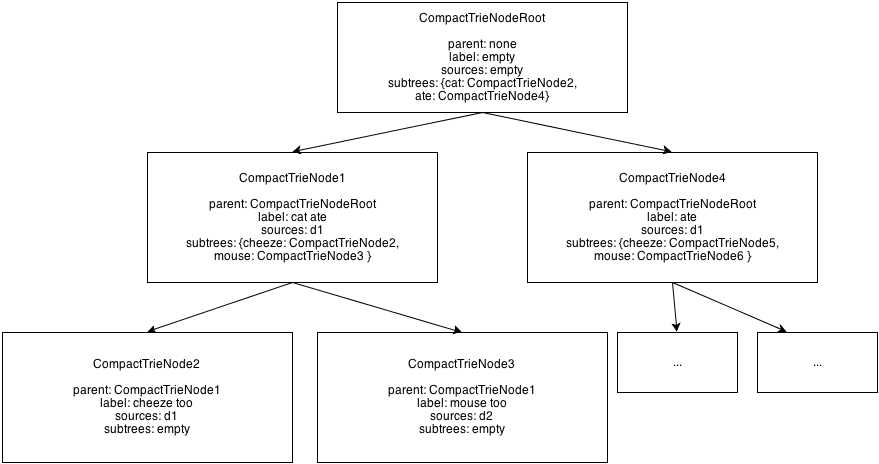
\includegraphics[totalheight=0.3\textheight]{Figures/compacttriedatastructure}
  \end{center}
  \caption{A simplified diagram of the compact trie data structure using two snippets “cat ate cheese” (d1) and “cat ate mouse too” (d2).}
  \label{fig:compacttriedatastructure}
\end{figure}

\subsubsection{Base clusters}

The \CTC algorithm generates base clusters with a simple recursive function. The function is called and applied to the root node of the compact trie. The function then creates new base clusters for each subtree in the root, and the subtrees of those subtrees etc. When all subtrees have been explored, the function iteratively adds the sources of each subtree to their parent base cluster as the function climbs out of the recursion. This way each base cluster's sources (given a node in the compact trie) is the union of all the sources in the decendant nodes.

The algorithm then sorts the base clusters according to their base cluster score. Recall the function for calculating the effective length of a base cluster label \(f(\vert P \vert)\) where \(f(\vert P \vert) = 0\) for \(\vert P \vert < 2\), \(f(\vert P \vert) = \vert P \vert\) for \(2 \le \vert P \vert < 7\), and \(f(\vert P \vert) = 7\) for \(7 < \vert P \vert\). Here the value 2 and 7 have been replaced by dynamic parameters min and max limits for base cluster scores. The min limit is a number in the range 1 \dots 5; the max limit a number in the range 3 \dots 9. If a corpus yields base clusters with generally longer labels, this will allow labels of longer lengths to be scored differently. A higher min limit will reduce the number of base clusters with short labels that might else wise be used in cluster creation.

TODO: Run analysis on base clusters produced to determine more optimal ranges.

The effective length of a label is dependent on the document frequency of each word in that label. A word contributes to a labels length if it satisfies two document frequency constraints. It should, according to \cite{Oren1998} have a document frequency of at least 4, and occur in no more than 40\% of the collection's documents. Because word frequencies vary in different corpora the optimal parameters for each of the limits might also vary. Each limit have thus been made dynamic. The first value ranges from 1 to 500, and the second from 0.1 to 1 with increments of 0.01.

\subsubsection{Base cluster merging and clusters}
Recall that \cite{Oren1998} merge base clusters using the Jaccard Coefficient on the number of shared documents, and each base clusters number of documents. This implementation is fairly naive because it only considers the amount of sources the base clusters share. This produces bigger clusters with good source overlap (number of shared sources), but runs the risk of producing clusters with low label overlap (few shared label words). In his research work \supervisor has implemented two new similarity functions which in addition to standard Jaccard Similarity considers the similarity of the base clusters' labels. 

One measure uses the vector space model and the cosine similarity function to find the similarity of base cluster labels. In this context a term's weight (tf-idf) is calculated not using it's document frequencies, but rather their base cluster frequencies. Given a base cluster \(b\), the concatenation \(S^+\) of \(b\)'s documents, and the corpus collection \(C\) the tf-idf score of a given term \(t\) in \(b\)'s label can be calculated with the function (insert cite to Richard's working paper?):

\begin{displaymath}
\vec{v}(t) = \left\{
  \begin{array}{l l}
    tf-idf(t, S^+, C) & \quad \text{if $t \in b$}\\
    0 & \quad \text{otherwise}
  \end{array} \right.
\end{displaymath}

Two base cluster labels are said to be similar if they satisfy the condition:

\begin{displaymath}
\frac{\sum_{t}\vec{v}(t) * \vec{v}'(t)}
{\sqrt{\sum_{t}\vec{v}(t)^2} * \sqrt{\sum_{t}\vec{v}'(t)^2}}
\ge \theta_{cos}
\end{displaymath}

where \(\theta_{cos}\) is the threshold with which similarity is determined. A \(\theta_{cos}\) close to 1 will prevent base clusters from being merged, whilst a value close to 0 would allow close to all Jaccard similar base clusters to be merged. Finding the right \(\theta_{cos}\) should therefore be part of the optimization task.

The second similarity measure used in \supervisor working paper is one of several amendments to the original Jaccard similarity measure used by \citeauthor{Oren1998}. Under this new similarity measure two base clusters are similar if: they are Jaccard similar, the average corpus frequency (\(cf(w)\)) of their label words are below some threshold (\(\theta avg\)), and that they share at minimum (\(\theta min\)) a number of label words. This amendment can be expressed mathematically as:

\begin{displaymath}
\frac{\sum\limits_{w \in b \cup b'} cf(w)}{\vert b \cup b' \vert} < \theta avg \quad \text{and} \quad \vert b \cap b' \vert > \theta min
\end{displaymath}

TODO: What does it try to capture?
This similarity measure aims to capture those base cluster pairs who's labels indicate that the merged cluster would be extremely general. That is base cluster pairs who's average corpus frequency are higher than some threshold considered average for the collection. The measure also attempts to filter out those clusters that does not share label words.
%\begin{lstlisting}[float=t, language=python, label=lst:clusteringcode, caption={Code}]
%
%\end{lstlisting}



\section{Testing}
\label{Testing}
During the thesis work, tests have been performed at various stages in order to justify the parameters selected and the value ranges for those parameters. Tests have also been performed to test the TODO: FIND TERM HERE of the genetic algorithm, distribution of computation and finally in the form of a scientific experiment to test the hypotheses posed in the thesis. This section will present a short overview of the informal tests and then go into some details about how the experiment was conducted and what kind of results were obtained. 

\subsection{Value Range Tests}
Describe tests to discover reasonable parameter ranges ...

\subsection{Genetic Algorithm Test}
Describe first test with about 200 individuals and 50 generations.

\subsection{Distributed Genetic Algorithm Test}
Describe distributed test with more individuals and more generations

\subsection{Final testing}
Describe final test and how it answers resesearch question.